\chapter{Test}

Projektet stiller krav om let udvikling og ikke mindst krav om kvalitet. Automatiserede tests har dermed været et naturligt valg, der konstant og systematisk hjæper os til at sørge for at kvaliteten i vores system opretholdes, foruden at hjælpe udviklingen til ikke at få detektere fejl i tidligere kode, når ny kode tillægges.

\section{Continous integration}
Der er i projektet anvendt Continuous Integration af systemet, således at når der pushes, så startes der automatisk en test af systemet.

\section{Continuous Integration}
Projektet er sat op, så der benyttes continuous integration, så projektet bliver bygget på en ekstern server, hver gang der bliver tilføjet en ændring til projektet via git. CI er blevet brugt for at undgå integrations problemer, der kan opstå, når flere gruppemedlemmer arbejder samtidig på samme projekt.
I forbindelse med at projektet bliver bygget på CI-serveren bliver de projektets test samtidig kørt.

TeamCity blev anvendt som CI-server, hvor der blev opsat et  projekt, der blev sat til at pege på gruppens github-repository. Projektet blev sat op til, at hver gang der blev "pushed" til reopistoriet skulle TeamCity kører to "Build Steps". I første step blev projektet bygget ved brug af MSBuild Tools 2015. Hvis det første skridt gik godt blev anden step udført, der bestod i at køre Test-projektets NUnit-tests. Testene blev kørt ved brug af en NUnit.ConsoleRunner, der var blevet installeret som en NuGet-Package i projektet.  
CI-projeket blev også tilknyttet en dotCover-test, der skulle fungere som et pejlemærke for, hvor stor en del af projektet testene dækker. Da der ikke var nogen specielle krav til Coverage-analysen blev JetBrains standard dotCover fil benyttet.

\noindent Nedenunder på figur \ref{fig:TeamCityTest} kan et eksempel af et build på TeamCity serveren ses. 
\begin{figure}[ht!]
	\centering
	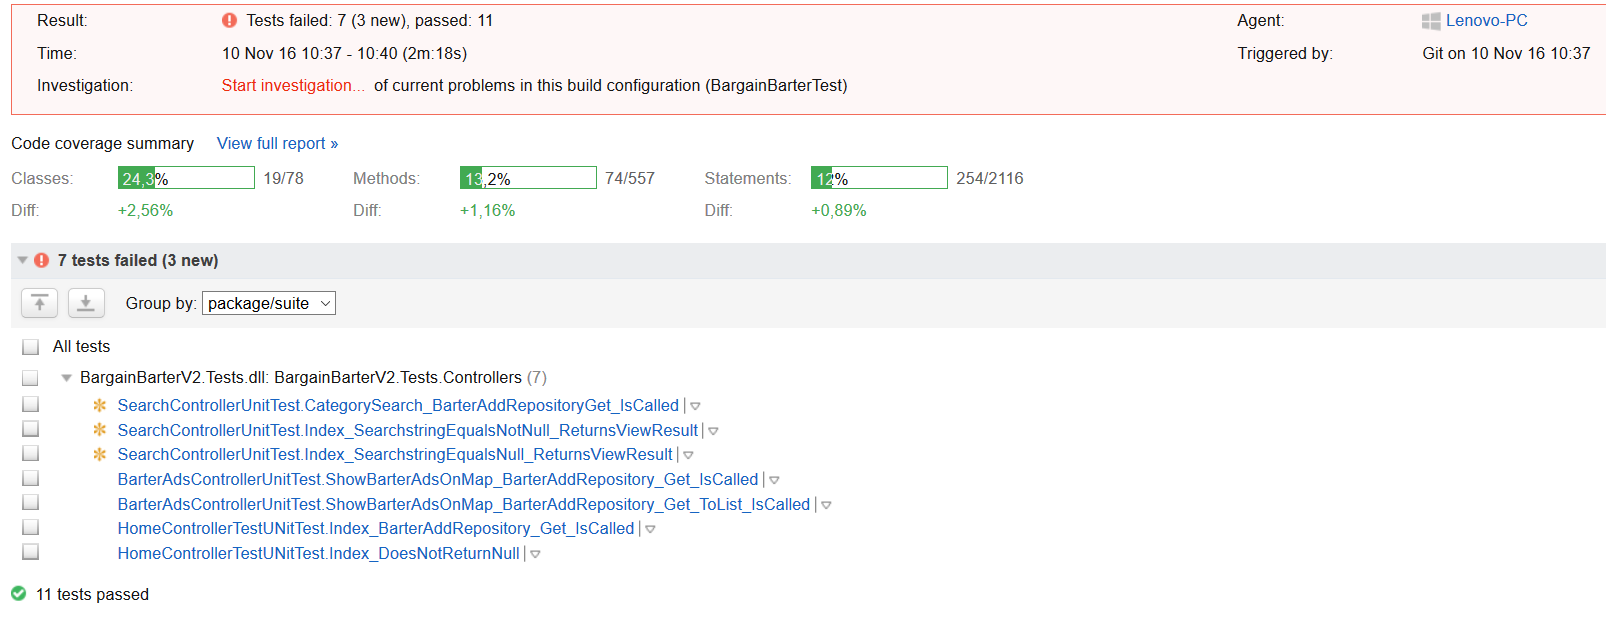
\includegraphics[width=120mm]{figures/TeamCityTest.png}
	\caption{Testresultat på baggrund af kørte test på TeamCity}
	\label{fig:TeamCityTest}
\end{figure}



\section{Unit Tests af controllerne}
Da der i Bargain Barter systemmet kun er meget minimal buisness-logic, ligger størstedelen af funktionaliteten i controllerne i MVC strukturen. Denne funktionalitet er således også den vigtigste at teste. Desuden er databasen i sig selv svær at teste, og views i MVC'en kan nærmest ikke testes. Det der reelt kan testes er hvad controllerne giver videre til deres views, og således ikke views dem selv. I Controllerne er der flere ting der er væsentligt at teste.
\begin{itemize}
	\item Hvad gives med i viewbagen
	\item Buisness-logic funktioner som controllerne bruger
	\item At de korrekte fejl bliver kaldt når controllerne giver ugyldige værdier
	\item De enkelte redirects bliver kaldt korrekt
	\item At de enkelte controllers returnerer views
\end{itemize}       
Disse er de udvalgte ting som er vurderet til at give mening at teste på.

Den fulde liste af test kan ses nedenfor.
(LAV DENNE LISTE!)
\setlength{\arrayrulewidth}{0.3mm}
\setlength{\tabcolsep}{2pt}
\renewcommand{\arraystretch}{1.5}
\begin{table}[H]
	\begin{tabular}{ | p{3.0cm} | p{5.5cm} | p{8.0cm} | }
		\hline
		\textbf{Controller} & \textbf{Test} & \textbf{Beskrivelse} \\
		\hline
		BarterAds-Controller &  Index\_RedirectsToController-\_HomeActionIndex & Tester om controlleren faktisk kalder der rigtige view til Home. \\
		
		& ShowBarterAdsOnMap-\_BarterAddRepository-\_Get\_IsCalled & Tester om controller kalder den rigtige metode for at vise alle barteradds på kortet\\
	
		& Details\_NullId\_Returns-\_BadRequest & Tester om hvis metoden Details får Null, som id, så returnerer controlleren en BadRequest, kode 400. \\
		\hline
		HomeController & Index\_BarterAddRepository-\_Get\_IsCalled & Tester om den metode der viser alle barteradds på Index siden, bliver vist. \\
		\hline
		SearchController & Search\_Calls-\_BarterAdsRepository & Tester om den BarterAddRepository bliver kaldt når man søger efter en bestemt ting \\
		& CategorySearch\_Calls-\_BarterAdsRepository & Tester om BarterAdsRepository anvendes at og bliver kaldt når man vælger kategori \\
		\hline
		
		
	\end{tabular}
\end{table}

Det er væsentligt at pointere hvordan disse test bliver lavet isoleret, således at controllerne ikke er afhængige af DAL-laget.

\subsection{Unit test igennem DAL}

Som nævnt spiller design og test i høj grad sammen, hvor der som nævnt er anvendt repository pattern. Hvor man på figur \ref{fig:UnitOfWorkMock} kan se at det i høj grad spiller sammen med test af systemmet. Det er muligt at teste systemmet direkte gennem db contexten som ses uden Repository pattern, men dette er ikke en selvfølgelighed, og ved ændring af database teknologi vil alle tests skulle skrives om. Dette er ikke ønsket, da selve unit testen skal teste om der sker kald ned i selve klassen, ikke om de kald rent faktisk virker. Det er ikke controllerne i MVC'en der har ansvar for at db kaldende virker. Derfor bruges en mock af den UnitOfWork som controlleren kalder ned i, og igennem repository patternet, opnås at controllerne kan testes uafhængigt af DAL laget og selve databasen.

\begin{figure}[H]
	\centering
	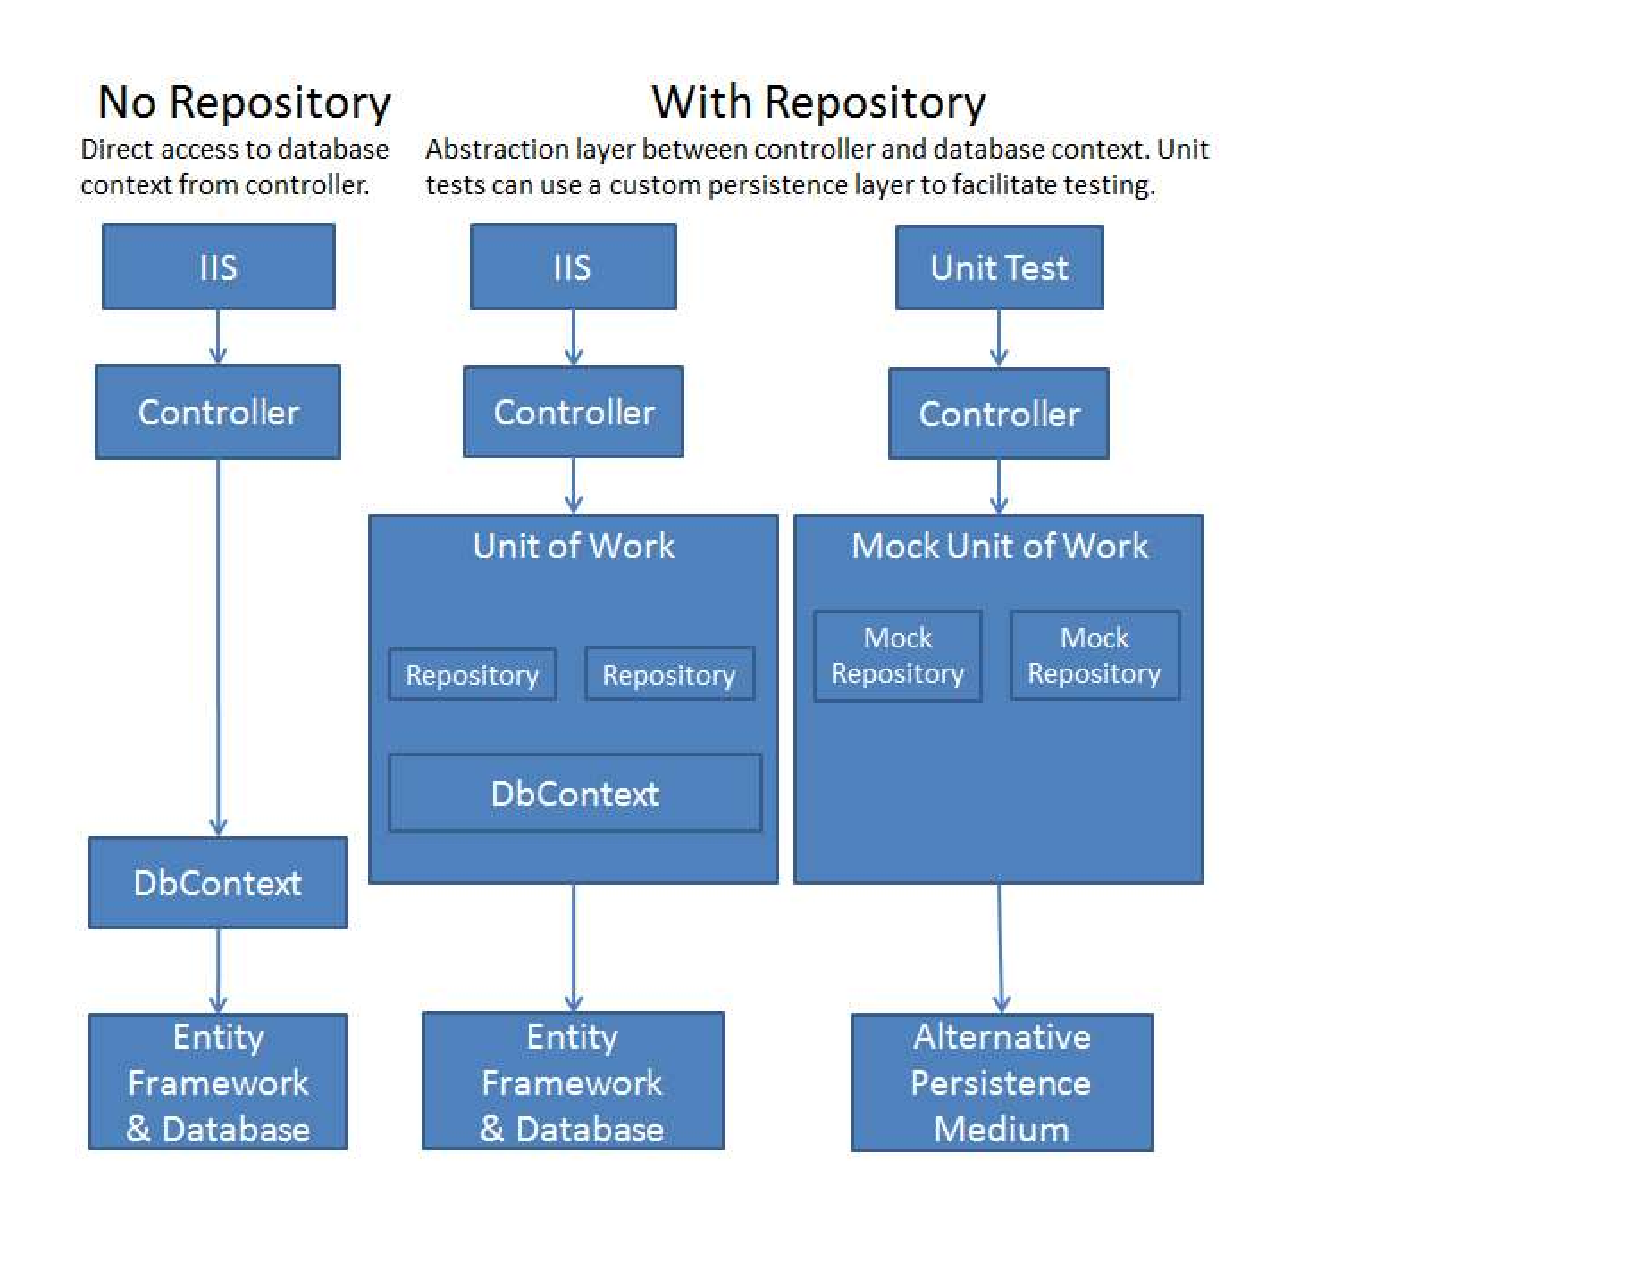
\includegraphics
	[width=165mm]{figures/RepsitoryTestFigure.PDF}
	\caption{Unit test med UnitOfWorkMock}
	\label{fig:UnitOfWorkMock}
\end{figure}

\section{Integrationstest}
%Efterfulgt af at de enkelte unit tests af controllersne, testes integrationen af controllerne med den relle database. Da samhørigheden af de forskellige controllers er forholdsvis lav er integrationstesten en relativ simpel opgave, hvor der kun er taget de enkelte dele der er vurderet til at give mening med.    
%
%INDSÆT DPTREE
%%\begin{figure}[H]
%%	\centering
%%	\includegraphics
%%	[width=165mm]{figures/DependencyTree.PDF}
%%	\caption{DependencyTree}
%%	\label{fig:DependencyTree}
%%\end{figure}
%
%\noindent Det sidste skridt er selvfølgelig at tests viewne, hvor der er lavet en user experience vurdering, og naturligvis en acceptest der kan ses i efterfølgende afsnit
Efterfulgt af unit test de enkelte controller, skal integrationen mellem de forskellige dele af systemet testes. Der er dog imidlertid ikke den store afhængighed mellem de forskellige controllers i systemet, hvilket MVC også lægger op til. Det ville derfor ikke give mening at lave en integrationstest af systemet, da der reelt er få dele af systemet, hvor man kan teste for afhængigheden mellem de forskellige dele af systemet. \\
